\documentclass[UTF8]{ctexart}

\usepackage{subfiles}  

%下面的语句, 引入你的头部设置文件
\usepackage{C:/phpStorm_proj/02_myself_ID_EGO/+100_latex_all_math_sel/myPreamble} 
%必须是绝对路径,才能让各个tex在单独编译时使用到

\title{文件名}


%---------------------------------


\begin{document}
	\tableofcontents % 生成目录
	\date{} % 若不写这句, 则默认也会渲染出日期, 所以我们要手动赋空值
	\maketitle  %这行代码, 让你前面的 title, author, date生效
	
	
	
	
	
	\section{传染病模型}
	
	
	\begin{myEnvSample}
		有红球a个, 黑球b个. 你从中取出一个球, 看到其颜色后, 把它放回, 并同时再放入c个与你看到的颜色相同的球. 	问:  连续3次都是取出红球的概率? \\
		先设定事件: \\
		- $A_1$ : 表示你第1次, 取出的是红球 \\
		- $A_2$ : 表示你第1次, 取出的是红球 \\	
		- $A_3$ : 表示你第3次, 取出的是红球 \\	
		
		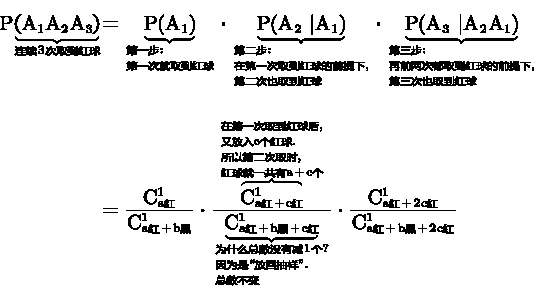
\includegraphics[width=0.85\textwidth]{/0094.pdf} \\
		
		上面可以看出: \\
		- 当 c红= 0 时, 就是正常的``放回抽样". \\
		- 当 c红= -1 时, 就是``不放回抽样". 即把之前步骤中取到的球, 拿走了, 不放回总体中. \\
		- 当 c红>0 时, 就是本例的``传染病模型".	
	\end{myEnvSample}
	
	
	
	
	
\end{document}